% !TEX root = dissertation_BB.tex
%% spellcheck-language en-US


  %#######  ########   #######   ######  
  %#     ## ##     ## ##     ## ##    ## 
  %#     ## ##     ## ##     ## ##       
  %#######  ########  ##     ## ##       
  %#        ##   ##   ##     ## ##       
  %#        ##    ##  ##     ## ##    ## 
  %#        ##     ##  #######   ######  

  \graphicspath{{./figures/3_processing/}}

  % \section{Image processing for light-sheet microscopy}
  
  %   necessary preprocessing steps for multi-view light-sheet microscopy
  %   image fusion
  %     1. bead based registration
  %     2. weighted average / cake fusion
  %     3. multi-view deconvolution
  
  \chapter{Image compression}
  \label{ch:compr}
    % As we will see later (\autoref{sec:sizes}), 
    Light-sheet microscopy is capable of generating an immense amount of data in a short amount of time. For this reason not only fast data processing, but data compression also plays an important role when evaluating, sharing and storing the images. In this chapter we will briefly introduce the core concepts of image compression and show some examples as a background for \autoref{ch:GPU}. For a more comprehensive review on data compression fundamentals, the interested reader is referred to the works of Sayood \cite{sayood_introduction_2012}, and Salomon and Motta \cite{salomon_handbook_2010}.
   
    There are two distinct ways of data compression: lossless and lossy. This is an important difference, and the choice between the two greatly depends on the application itself. For some types of data no loss is acceptable, for example computer programs or text. Here, even a small change could drastically influence the meaning of the original data. For other applications, such as audio and video compression, some loss can be tolerated as long as there is no perceived change or distortion. For scientific applications mostly lossless compression is used. Even for image data, where lossy compression can significantly increase the compression ratio (original size / compressed size), lossy compression is usually not recommended, as it can alter the measurement results in unpredictable ways \cite{cromey_digital_2013}.
  
    % There are a multitude of techniques developed in the context of data compression, and most compression methods are built based on this repertoire. Because of this, many algorithms follow a common pattern, and 
  
    \section{Basics of information theory}
      \label{sec:entropy}
      As compression is the art of reducing the size of a message while keeping the same amount of information, it is necessary to briefly discuss the theory behind information, and how to quantify it. These concepts were first introduced by Shannon, in his highly influential papers \cite{shannon_mathematical_1948,shannon_mathematical_1948-1,shannon_prediction_1951}. As a rigorous mathematical explanation is outside the scope of this work, we refer the interested reader to the aforementioned works.
  
      Informally, information can be quantified as the amount of surprise. A statement, if it has a high probability, carries a low amount of information, while if it has a small probability, there is more information. Consider the following example: ``It is July". If it is indeed July, this statement doesn't provide too much information. Continuing with ``It is snowing outside", carries more information, as it is unexpected under the circumstances (provided the conversation takes place on the Northern Hemisphere).
  
      The self-information of event $A$ can be defined the following way:
      \begin{equation}
        I(A) = \log_b \frac{1}{P(A)} = - \log_b P(A),
        \label{eq:selfInfo}
      \end{equation}
      where $P(A)$ is the probability of event $A$ occurring. The base of the logarithm can be chosen freely, but usually the preferred base is $b=2$. With this choice, the unit of information is \SI{1}{bit}, and $I(A)$ represents how many bits are required to store the information contained in $A$.
  
      The average self-information, also called entropy, for a random variable $X$ can be calculated based on the self-information of the outcomes $A_i$:
      \begin{equation}
        H(X) = \sum_i P(A_i)I(A_i) = - \sum_i P(A_i) \log_b P(A_i)
        \label{eq:entropy}
      \end{equation}
      If we consider a data stream $S$, where each symbol records the outcome of independent, identical random experiments $X$, then the average information in each symbol will be $H(X)$. As a consequence, as stated by Shannon's source coding theorem \cite{shannon_mathematical_1948}, the shortest representation of $S$ will require at least $N\cdot H(X)$ bits, where $N$ is the number of symbols in the stream. This defines the theoretical lower bound that any na\"ive compression algorithm, also called entropy coding, can achieve without loosing any information.
  
      The requirement, however, is that the symbols are independent of each other, which is usually not true for most of the data types we (humans) are interested in. In order to achieve ideal compression, the input needs to be modeled, or transformed, to represent it as a sequence of independent variables. This pattern of modeling and coding \cite{rissanen_universal_1981} is the core of all modern compression algorithms. 
      The following sections will briefly introduce these concepts by two examples: Huffman coding, and pixel prediction.
      
      % in the context of image compression
      % redistributing probabilities
      
    \section{Entropy coding}
      \label{sec:entropyCoding}

      Entropy coding algorithms aim to reduce data size and reach the limit of entropy for any kind of input based on the probability distribution of the possible symbols. All of these algorithms work in a similar way, as their aim is to represent the symbols of the input data by codewords in a way to minimize the overall length of the data. Variable length codes, for example, replace the more common symbols with short codewords, while for less frequent symbols they use longer codewords. The ideal length of a codeword for symbol $A$ is actually equal to $I(A)$, as this was the definition of self-information.


      \subsubsection{Prefix-free codes}

      Fixed-length codes have the convenience that there is no need to indicate the boundaries between them, as they are all the same length (\textit{e.g.}, \SI{8}{bits} for ASCII codes). For variable length codes, as the name implies this is not possible, which necessitated the development of various strategies to demarcate these codewords. 

      One way to indicate the end of a codeword is to use a specific delimiting sequence which is not part of any of the codewords. While this is an obvious solution, it is also wasteful, as these sequences will not contain any information regrading the original source. Prefix-free codes were developed to be able to omit these sequences, while still allowing unique decodability, making them very popular. This is achieved by making sure that once a codeword was assigned, no other codeword would start with that sequence. In other words, no codeword is a prefix of another codeword, hence the name of the technique. During decoding the bits are read until a valid codeword is matched. Since it is guaranteed that no other codeword will start with the same sequence, the decoder can record the symbol corresponding for that codeword, and continue reading the compressed stream.
      % A practical implementation to this process is based on representing the codewords in a binary tree where each edge corresponds to one bit and is labeled 1 or 0. As the decoder is reading the bits, it traverses down the tree until it reaches a leaf. The symbol represented by that leaf will be the decoded symbol and the process can start over from the beginning.
      
      Let's take the example in \autoref{tab:prefix}. Five letters are coded in binary code by Code \#1 and by Code \#2. Code \#1 is not a prefix code, and because of this when reading the encoded sequence we can not be sure when we reach the end of a codeword. Decoding the sequence 0000 for example could be interpreted as 4 letters of $a_1$ or 2 letters of $a_3$. For Code \#2 it is clear that the sequence decodes to 2 letters of $a_3$.
  
      \begin{table}
        \bcaption[Examples of a random binary code (\#1) and a prefix-free binary code (\#2)]{Code \#2 is uniquely decodable, while for code \#1 it is necessary to introduce boundaries between codewords to be able to distinguish them.}
        \centering
        \begin{tabular}{crr}
          \toprule
          Letter & Code \#1 & Code \#2 \\
          \midrule
          $a_1$ & 0	& 10 \\
          $a_2$ & 11	& 11 \\
          $a_3$ & 00	& 00 \\
          $a_4$ & 10 	& 010 \\
          $a_5$ & 111	& 011 \\
          \bottomrule
        \end{tabular}
        \label{tab:prefix}
      \end{table}
  
      % how to reduce data size? use variable length codes
      % code length depends on symbol frequency - more frequent, shorter codes
      % problem? how do we know the boundaries between codewords?
      % prefix free codes - no codeword is a prefix of any other codeword
      % Huffman coding is like this, and also ideal in the sense that the average codeword length for large data
      % "The long discussion in [Gilbert and Moore 59] \cite{gilbert_variable-length_1959} proves that the Huffman code is a minimum-length code in the sense that no other encoding has a shorter average length"
  

      \subsubsection{Huffman coding}

      Huffman coding is a prefix-free, optimal code that is widely used in data compression. It was developed by David A. Huffman as a course assignment in the first ever course on information theory at MIT, and was published shortly afterwards \cite{huffman_method_1952}. It is able to achieve optimal compression in a sense that no other prefix-free codes will produce a shorter output. Due to its simplicity combined with a good compression ratio it is still widely used in many compression algorithms, such as in JPEG, bzip2, or DEFLATE (zip) \cite{salomon_handbook_2010}.
      
  
      The Huffman coding procedure is based on two observations regarding optimal and prefix-free codes:
      \begin{enumerate}
        \item For a letter with higher frequency the code should produce shorter codewords, and for letters with lower frequency it should produce longer codewords.
        \item In an optimum code, the two least frequent codewords should have the same lengths.
      \end{enumerate}
  
      From these statements it is trivial to see that the first is correct. If the more frequent letters would have longer codewords than the less frequent letters, then the average codeword length (weighted by the probabilities) would be larger than in the opposite case. Thus, more frequent letters must not have longer codewords than less frequent letter.
  
      The second statement at first glance might not be so intuitive, so let's consider the following situation. Let's assume that the two least frequent codewords do not have the same lengths, and the least frequent is longer. However, because this is a prefix code, the second longest codeword is not a prefix of the longest codeword. This means that if we truncate the longest codeword to the same length as the second longest, they will still be distinct codes and uniquely decodable. This way we have a new coding scheme which requires less space on average to code the same sequence as the original code, from which we can conclude the original code was not optimal. Therefore, for an optimal code, statement 2 must be true.
  
      \begin{table}
        \bcaption[Letters to be Huffman coded and their probabilities]{}
        \centering
        \begin{tabular}{ccr}
          \toprule
          Letter & Probability & Codeword \\
          \midrule
          $a_2$ & 0.4 & $c(a_2)$ \\
          $a_1$ & 0.2 & $c(a_2)$ \\
          $a_3$ & 0.2 & $c(a_2)$ \\
          $a_4$ & 0.1 & $c(a_2)$ \\
          $a_5$ & 0.1 & $c(a_2)$ \\
          \bottomrule
        \end{tabular}
        \label{tab:huffman1}
      \end{table}
  
      \begin{figure}
        \centering
        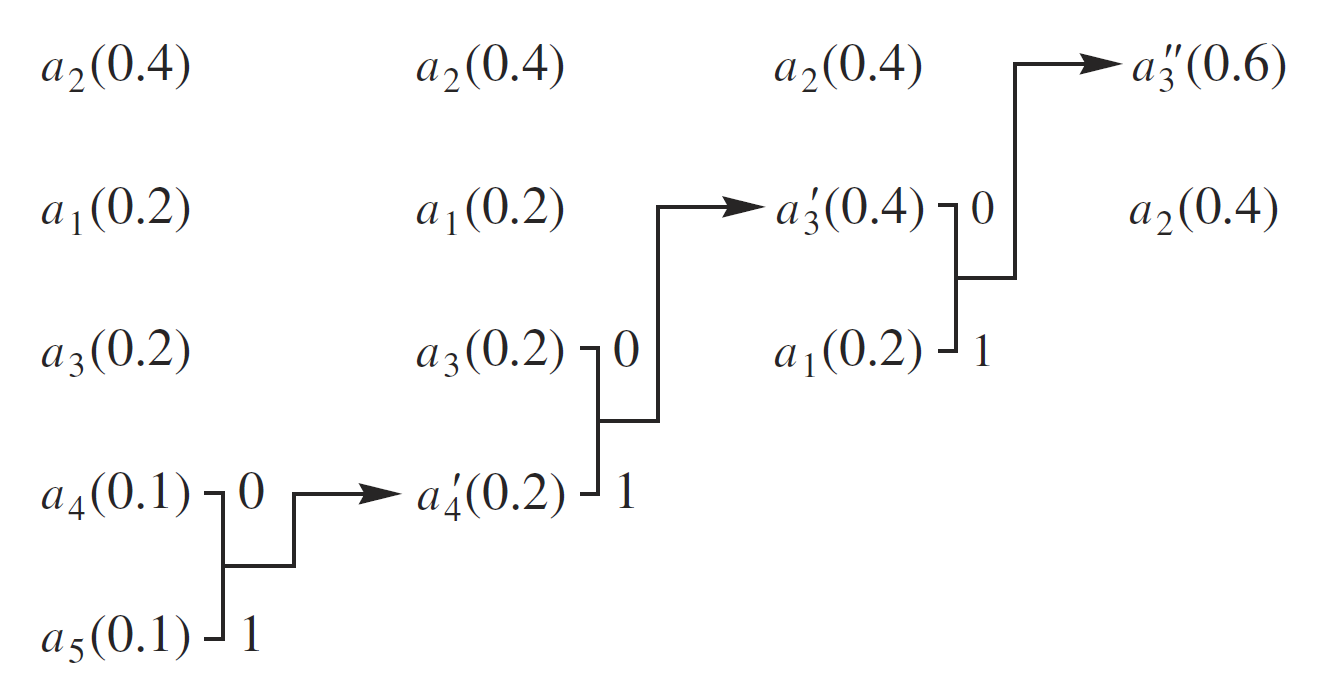
\includegraphics[width=0.6\textwidth]{huffman}
        \bcaption[Building the binary Huffman tree]{The letters are ordered by probability, these will be the final leaves of the tree. To create the branches, at every iteration we join the two nodes with the smallest probability, and create a new common node with the sum of the probabilities. This process is continued until all nodes are joined in a root node with probability of 1. Now, if we traverse down the tree to each leaf, the codeword will be defined by their position.}
        \label{fig:huffman}
      \end{figure}
  
      To construct such a code, the following iterative procedure can be used. Let's consider an alphabet with five letters $A = [a_1,a_2,a_3,a_4,a_5]$ with $P(a_1)=P(a_3)=0.2$, $P(a_2)=0.4$ and $P(a_4)=P(a_5)=0.1$ (\autoref{tab:huffman1}). This distribution represents a source with 2.122 bits/symbol. Let's order the letters by probability, and consider the two least frequent. Since the codewords assigned to these should have the same lengths, they can be assigned as
      \begin{align*}
        c(a_4) &= \alpha_1 * 0 \\
        c(a_5) &= \alpha_1 *1
      \end{align*}
  
      where $c(a_i)$ is the assigned codeword for letter $a_i$ and $*$ denotes concatenation. Now we define a new alphabet $A'$ with only four letters $a_1, a_2, a_3, a'_4$, where $a'_4$ is a merged letter for $a_4$ and $a_5$ with the probability $P(a'_4) = P(a_4) + P(a_5) = 0.2$. We can continue this process of merging the letters until all of them are merged and we have only one letter left. Since this contains all of the original letters, its probability is 1. We can represent the end result in a binary tree (see \autoref{fig:huffman}), where the leaves are the letters of the alphabet, the nodes are the merged letters, and the codewords are represented by the path from the root node to each leaf (compare with \autoref{tab:huffman2}). The average length of this code is
      \begin{equation}
        l = 0.4\times 1 + 0.2 \times 2 + 0.2 \times 3 + 0.1 \times 4 + 0.1 \times 4 = 2.2 \text{ bits/symbol}
      \end{equation}
      The efficiency of a code can be measured by comparing the average code size to the entropy of the source. For this example, the difference is 0.078 bits/symbols. As the Huffman code operates in base 2, it will produce a code with zero redundancy when the probabilities are negative powers of 2.
  
      \begin{table}
        \bcaption[Huffman code table]{}
        \centering
        \begin{tabular}{ccr}
          \toprule
          Letter & Probability & Codeword \\
          \midrule
          $a_2$ & 0.4 & 1 \\
          $a_1$ & 0.2 & 01 \\
          $a_3$ & 0.2 & 000 \\
          $a_4$ & 0.1 & 0010 \\
          $a_5$ & 0.1 & 0011 \\
          \bottomrule
        \end{tabular}
        \label{tab:huffman2}
      \end{table}

    \subsubsection{Limitations of Huffman coding}
      Although the Huffman code is optimal among variable-length codes, for certain types of data its compression ratio may be low. This limit lies in the fact that the length of the shortest code assignable is one. For certain types of data with very low entropy this will result in a relatively high redundancy. Arithmetic coding offers an alternative here, as contrary to Huffman coding, it does not rely on substituting symbols with codewords, and thus can compress very low entropy data with minimal redundancy. This coding method maps the whole message to a single number with arbitrary precision in the interval of 0 to 1. A more detailed description of arithmetic coding in given in \cite{sayood_introduction_2012}.

      Another alternative for compressing very low entropy data is run-length encoding. This coding method assumes that the same character appears in the message many times consecutively, and instead of storing each of these individually, it counts the number of identical symbols in a single run, and encodes the run-length together with the symbol. As this strategy is only efficient for very low entropy data, it is a common practice to combine run-length encoding with Huffman coding to construct a low redundancy coder for a wide range of input data.
  
    \section{Decorrelation}
      \label{sec:decorrelation}
      Since entropy coding doesn't assume anything about the data structure, it is not capable of recognizing and compressing any regular patterns or correlations between the consecutive data points. To maximize the efficiency of compression, any correlations should be removed from the data before it is fed to the entropy coder. Here we will briefly discuss some decorrelation strategies for image compression that aim to improve the performance of a successive entropy coder.

      \subsubsection{Transform coding}
      Very popular methods for decorrelation are the transformations that represent the data as a decomposition of orthonormal functions. One of the most common of these transformations is the Fourier transform, which represents a periodic signal as a sum of sine an cosine functions. As most natural images are of continuous tone, the idea behind this is that most of the information will be captured by just a few Fourier coefficients. As a result, compressing the coefficients with an entropy coder should result in a smaller output than encoding the original data.

      For practical purposes, instead of the discrete Fourier transform (DFT), the discrete cosine transform (DCT) \cite{ahmed_discrete_1974} is usually used in image compression applications. This is very similar to DFT, the difference being the periodic extension of the signal. In the DCT transform the image is mirrored on the sides instead of just repeated, to avoid large jumps at the boundaries that may introduce unwanted high-frequency components in the Fourier transform. If the image is extended in a symmetric way, the Fourier transform will be able to represent the data with only cosine functions, hence the name discrete cosine transformation.

      One drawback of frequency-based transformations is that they can not capture any spatial information, as their base functions are periodic for the whole domain. This can have a negative impact on image compression ratio. For example, if the image contains a single sharp edge, a high frequency base function will need to have a large coefficient. Since this will affect the entire image, other, lower frequency bases will also need to have increased coefficients to negate the unwanted effects.
      To overcome this limitation, the DCT is usually performed on small chunks of the image, such as on 8\texttimes8 blocks in the JPEG compression. The other option is to use non-periodic base functions to represent the signal. One good example for this is the use of wavelets, and based on this, the discrete wavelet transform (DWT) \cite{mallat_theory_1989, jensen_ripples_2001}.

      As both DCT and DWT operate with floating-point coefficients (although DWT has integer-based variants), the inverse transformation is not guaranteed to exactly reconstruct the original data. This is due to the finite machine precision of floating-point numbers. Due to this fact these transformations are generally used in lossy compression algorithms, and the coefficients are quantized based on the required image quality.
      
      % Decorrelation itself does not compress the data, it just reorganizes the information in a way that make a subsequent entropy coder more efficient.
      
  
      \subsubsection{Predictive decorrelation}
      \label{sec:predictors}
      Another family of decorrelation methods is based on predicting the values of each data point (or pixel) depending on the context of the neighboring values. These techniques are based on differential pulse code modulation (DPCM), a decorrelation method originally used for audio compression. Here, before the data stream is entropy coded, a prediction is made for each value, which is equal to the preceeding value. The difference to the prediction, called the prediction error, or prediction residual ($\varepsilon$) is passed to the entropy coder.

      To see how why such an algorithm can increase compression ratio, let's consider the following sequence:
      \begin{center}
        \begin{tabular}{|c|c|c|c|c|c|c|c|c|c|c|c|c|}
          \hline
          37 & 38 & 39 & 38 & 36 & 37 & 39 & 38 & 40 & 42 & 44 & 46 & 48 \\
          \hline
        \end{tabular}
      \end{center}
      Although there is no obvious pattern in this sequence, there are no sharp jumps between the consecutive values, and this can be exploited by using a prediction scheme. Let's define the prediction $\Pred(\cdot)$ for each element $X_k$ to be equal to the preceding element. The prediction error would be $\varepsilon_k = X_K - \Pred(X_k) = X_k - X_{k-1}$:
      \begin{center}
        \begin{tabular}{|c|c|c|c|c|c|c|c|c|c|c|c|c|}
          \hline
          37 & 1 & 1 & -1 & -2 & 1 & 2 & -1 & 2 & 2 & 2 & 2 & 2 \\
          \hline
        \end{tabular}
      \end{center}
      As apparent from this new sequence, the number of distinct values are reduced, which means that fewer bits can represent this sequence than the original. When running these two sequences through an entropy coder, the error sequence will be much more compressed due to this property.
      
      Using a predictive scheme to remove correlations from neighboring elements is a very good strategy for various applications where this signal is only slowly changing. It has been successfully implemented in audio and image compression algorithms as well, such as lossless-JPEG \cite{pennebaker_jpeg:_1992}, JPEG-LS \cite{weinberger_loco-i_2000}, CALIC \cite{wu_context-based_1997}, SFALIC \cite{starosolski_simple_2007} and FLIC \cite{wang_fast_2012}, just to name a few.
  
      \begin{figure}
        \centering
        \renewcommand{\arraystretch}{1.5}
        \begin{tabular}{|c|c|c|c|c}
          \hline
          \rowcolor{gray!25}
          \ \ \ & \ & \ & \ \ \ & \ \\ \hline
          \rowcolor{gray!25}
          \ & C & B & D & \ \\ \hline
          \cellcolor{gray!25} \ & \cellcolor{gray!25}A & \cellcolor{green!25}X & \ & \ \\ \hline
          \ & \ & \ & \ & \ \\
        \end{tabular}
        \bcaption[Context for pixel prediction]{X is the current pixel to be encoded and the previously encoded pixels are indicated with gray background. To allow for decoding, only the already encoded pixels are used for the prediction, typically the nearest neighbors (A, B, C, D).}
        \label{fig:context}
      \end{figure}

      For image compression, as the datasets are inherently multi-dimensional, the prediction rules can also be multi-dimensional, which can better capture the structure of the data, and achieve better decorrelation. For a typical encoding scenario, where the pixels are encoded one by one, the prediction can be based on the already encoded values (gray in \autoref{fig:context}). This causality constraint is necessary in order to be able to decode the image.

      Usually the nearest neighbors are used for the prediction, but this is not a necessity; CALIC, for example, uses the second neighbors \cite{wu_context-based_1997}, and the third dimension can also be utilized if the data structure allows this, for example when encoding hyperspectral recordings \cite{aranki_hardware_2009}.

      The lossless part of the JPEG standard specifies 7 possible rules for the prediction step \cite{pennebaker_jpeg:_1992}:
      \begin{align*}
        \Pred_1(X) =& A \\
        \Pred_2(X) =& B \\
        \Pred_3(X) =& C \\
        \Pred_4(X) =& A + B - C \\
        \Pred_5(X) =& A + (B - C)/2 \\
        \Pred_6(X) =& B + (A - C)/2 \\
        \Pred_7(X) =& (A + B)/2 \\
      \end{align*}
      Depending on the patterns of the input image, some predictors can perform better than others. For general use, predictor 4 or 7 are recommended, as these are not direction dependent, and usually perform best. Predictor 7 is just the mean of the top and left neighbors, while predictor 4 assumes that the values for pixels A, B, C and X are on the same plane, and calculates the prediction based on this. 

      Other algorithms try to improve the prediction by adapting it depending on the local texture. The LOCO-I algorithm (part of JPEG-LS), for example, uses the median edge detector \cite{weinberger_loco-i_2000}:
      \begin{equation}
        \Pred(X) = 
        \begin{cases}
          \min(A,B) & \text{if } \geq \max(A,B) \\
          \max(A,B) & \text{if } \leq \min(A,B) \\
          A + B - C & \text{otherwise }
        \end{cases}
      \end{equation}
      This function tries to estimate if there is an edge close to X. If it detects a vertical edge to the left of X, it picks B for the prediction, whereas if it detects a horizontal edge above X it tends to pick A. If no edge is detected, the prediction is the same as predictor 4 of the lossless JPEG standard.

      A useful property of the prediction-based methods is that there is no base change as in the transform coding methods, and it is possible to construct bounded lossy compression algorithms. JPEG-LS, for example defines a near-lossless mode of operation, where the user can select the maximum absolute reconstruction error per pixel. This is achieved by quantizing the prediction residual $\varepsilon$ with a quantization step depending on the allowable error. Since the decoding algorithm simply calculates $\hat{X} = \pred(X) + \varepsilon$, any quantization error of $\varepsilon$ is directly reflected in the reconstructed pixel value. Since the quantization error is known, and bounded by the quantization step size, the maximum reconstruction error for each pixel is also bounded. This mode is sometimes used for medical imaging applications, where the preservation of diagnostic quality is required by law, but higher compression ratios are desired than what is possible by lossless compression.
  
  
  
  
  % \section{Noise in light microscopy images}
  % \subsection{Photon shot noise}
  % \subsection{Camera noise}
  %   \subsubsection{CCD}
  %   \subsubsection{EM-CCD}
  %   \subsubsection{sCMOS}
  % \subsection{Variance stabilization}
  